\documentclass{article}

\usepackage{fancyhdr}
\usepackage{extramarks}
\usepackage{amsmath}
\usepackage{amssymb}
\usepackage{amsthm}
\usepackage{amsfonts}
\usepackage{tikz}
\usepackage[plain]{algorithm}
\usepackage{algpseudocode}
\usepackage{graphicx}
\usepackage{forest}
\usepackage{pdfpages}
\usepackage{catchfile}
\usepackage{hyperref}

\topmargin=-0.45in
\evensidemargin=0in
\oddsidemargin=0in
\textwidth=6.5in
\textheight=9.0in
\headsep=0.25in


\linespread{1.1}

\pagestyle{fancy}

\lhead{Joel Ho Eng Kiat A0200385N}
\chead{CS3219}
\rhead{Task F}
\lfoot{\lastxmark}
\cfoot{\thepage}

\begin{document}
    Link to GitHub repo \href{https://github.com/JoelHo/cs3219-assignments/tree/master/task_f}{https://github.com/JoelHo/cs3219-assignments/tree/master/task\_f}\\

    Start a redis server in docker:

    \texttt{docker run --name a-redis -p 6379:6379 -d redis}

    Install deps, start the server:

    \texttt{npm install}

    \texttt{npm start}\\

    On the regular endpoint (104ms):

    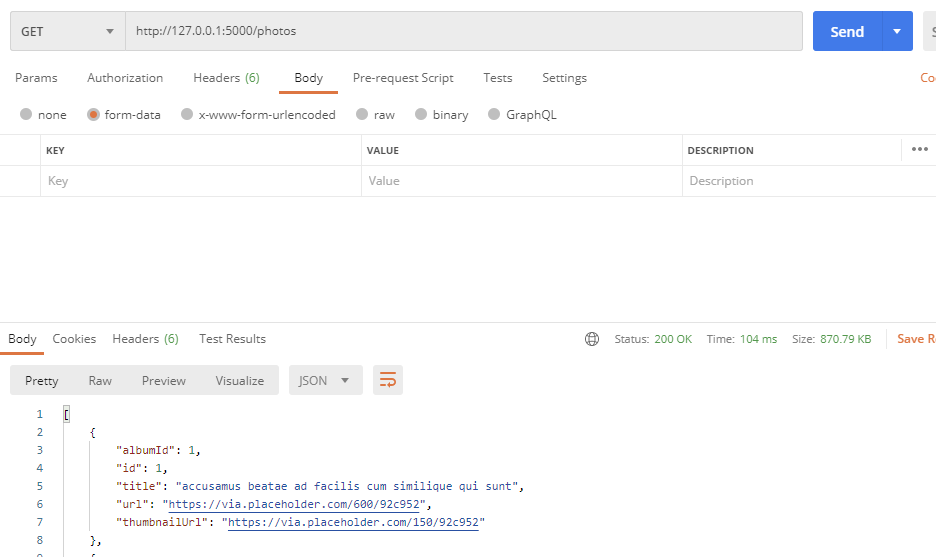
\includegraphics[width=\textwidth]{img/uncache.png}\\

    \pagebreak
    On the cached endpoint, first hit (147ms):

    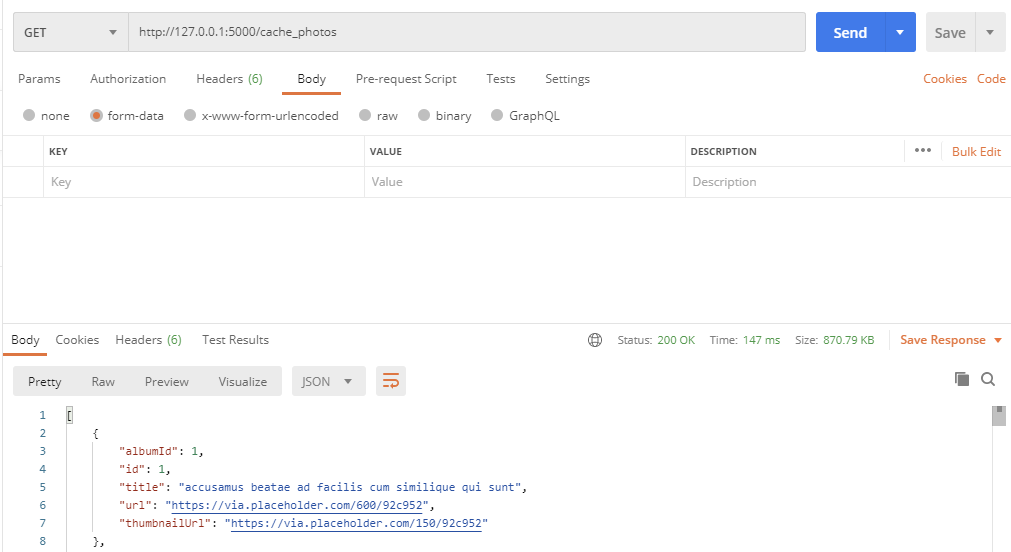
\includegraphics[width=\textwidth]{img/setcache.png}\\

    On the cached endpoint, next hit (66ms):

    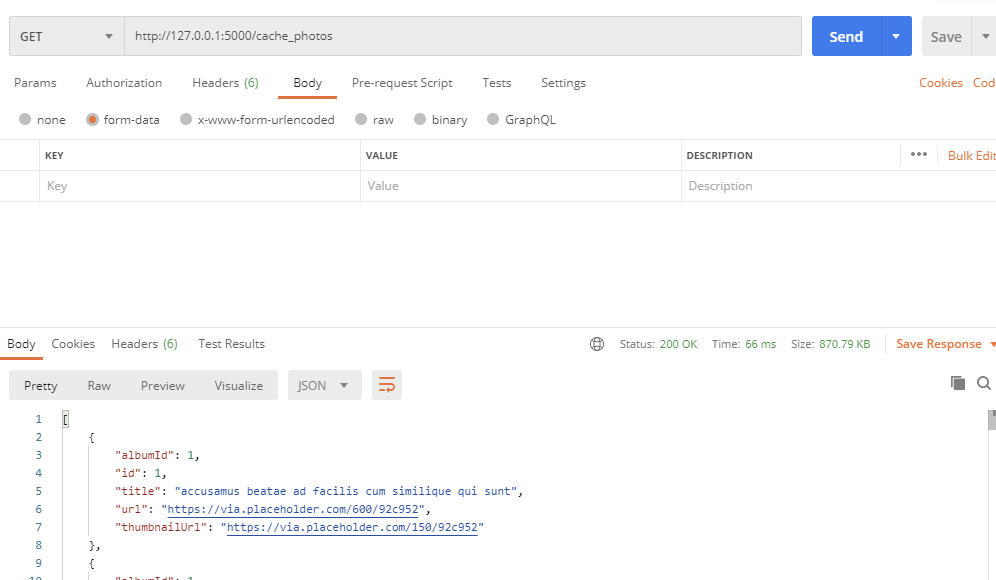
\includegraphics[width=\textwidth]{img/getcache.png}\\



\end{document}
